\documentclass[a4paper, 11pt, oneside, oldfontcommands]{memoir}

%%%%% Packages %%%%%
\usepackage{lmodern}
\usepackage{palatino}
\usepackage[T1]{fontenc}
\usepackage[utf8]{inputenc}
\usepackage[french]{babel}


%%%%%%%%%%%%%%%%%%%%  PACKAGE SECONDAIRE

%\usepackage{amstext,amsmath,amssymb,amsfonts} % package math
%\usepackage{multirow,colortbl}	% to use multirow and ?
%\usepackage{xspace,varioref}
\usepackage[linktoc=all, hidelinks]{hyperref}			% permet d'utiliser les liens hyper textes
\usepackage{float}				% permet d ajouter d autre fonction au floatant
%\usepackage{wrapfig}			% permet d avoir des image avec texte coulant a cote
%\usepackage{fancyhdr}			% permet d inserer des choses en haut et en bas de chaque page
\usepackage{microtype}			% permet d ameliorer l apparence du texte
\usepackage[explicit]{titlesec}	% permet de modifier les titres
\usepackage{graphicx}			% permet d utiliser les graphiques
\graphicspath{{./images/}}		% to say where are image
%\usepackage{eso-pic} 			% to put figure in the background
\usepackage[svgnames]{xcolor}	% permet d avoir plus de 300 couleur predefini
%\usepackage{array}				% permet d ajouter des option dans les tableaux
%\usepackage{listings}			% permet d ajouter des ligne de code
%\usepackage{tikz}				% to draw figure
%\usepackage{appendix}			% permet de faire les index
%\usepackage{makeidx}			% permet de creer les index
%\usepackage{fancyvrb}			% to use Verbatim
%\usepackage{framed}				% permet de faire des environnement cadre
%\usepackage{fancybox}			% permet de realiser les cadres
\usepackage{titletoc}			% permet de modifier les titres
%\usepackage{caption}
%\usepackage[a4paper, top=2cm, bottom=2cm]{geometry}
\usepackage{frbib}                      %permet d avoir une biblio francaise
\usepackage[babel=true]{csquotes}
\usepackage{eurosym}

\usepackage{graphicx}
\RequirePackage{pageGardeEnsta}	% permet d avoir la page de garde ensta

%\setcounter{secnumdepth}{2}		% permet d'augmenter la numerotation
%\setcounter{tocdepth}{2}		% permet d'augmenter la numerotation

%%%%%%%%%%%%%%%%%%  DEFINITION DES BOITES
\newcounter{rem}[chapter]

\newcommand{\remarque}[1]{\stepcounter{rem}\noindent\fcolorbox{OliveDrab}{white}{\parbox{\textwidth}{\textcolor{OliveDrab}{
\textbf{Remarque~\thechapter.\therem~:}}\\#1}}}

\newcounter{th}[chapter]

\newcommand{\theoreme}[2]{\noindent\fcolorbox{FireBrick}{white}{\stepcounter{th}
\parbox{\textwidth}{\textbf{\textcolor{FireBrick}{Théorème~\thechapter.\theth~:}}{\hfill \textit{#1}}\\#2}}}

\newcommand{\attention}[1]{\noindent\fcolorbox{white}{white}{\parbox{\textwidth}{\textcolor{FireBrick}{
\textbf{Attention !}}\\\textit{#1}\\}}}
%%%%%%%%%%%%%%%%%%%%%%%%%%%%%%%%%%%%%%%%%%%%%%%%%%%%%%%%%%%%%%%%%%%%%%%%%


%% INDEX %%%%%%%%%%%%%%%%%%%%%%%%%%%%%%%%%%%%%%%%%%%%%%%%%%%%
\makeindex

%%%%% Useful macros %%%%%
\newcommand{\latinloc}[1]{\ifx\undefined\lncs\relax\emph{#1}\else\textrm{#1}\fi\xspace}
\newcommand{\etc}{\latinloc{etc}}
\newcommand{\eg}{\latinloc{e.g.}}
\newcommand{\ie}{\latinloc{i.e.}}
\newcommand{\cad}{c'est-à-dire }
\newcommand{\st}{\ensuremath{\text{\xspace s.t.\xspace}}}

%%%% Definition des couleur %%%%

\newcommand\couleurb[1]{\textcolor{SteelBlue}{#1}}
\newcommand\couleurr[1]{\textcolor{DarkRed}{#1}}


%% number page style style %%%%%%%%%%%%%%%%%%%%%%%%%%%%%%%%%%%%%%%%%%%%%%%%%%%%%%

\pagestyle{plain}
%\pagestyle{empty}
%\pagestyle{headings}
%\pagestyle{myheadings}



%% chapters style %%%%%%%%%%%%%%%%%%%%%%%%%%%%%%%%%%%%%%%%%%%%%%%%%%%%%%
%% You may try several styles (see more in the memoir manual).

%\chapterstyle{veelo}
%\chapterstyle{chappell}
%\chapterstyle{ell}
%\chapterstyle{ger}
%\chapterstyle{pedersen}
%\chapterstyle{verville}
\chapterstyle{madsen}
%\chapterstyle{thatcher}


%%%%% Report Title %%%%%
\title{Rapport}
\author{\textsc{Équipe Smart:}\\D'Acremont Antoine\\Cotten Guillaume\\Legay Kevin\\Kennan Aya\\Shehade Mohammed\\Rigaud Michaël}
\date{\today}
%\doctype{Rapport}
\promo{promo 2017}
\version{2.0}
\etablissement{\textsc{Ensta} Bretagne\\2, rue François Verny\\
  29806 \textsc{Brest} cedex\\\textsc{France}\\Tel +33 (0)2 98 34 88 00\\ \url{www.ensta-bretagne.fr}}
\logoEcole{
\includegraphics[height=4.2cm]{logo_ENSTA_Bretagne_Vertical_CMJN}}
\logoun{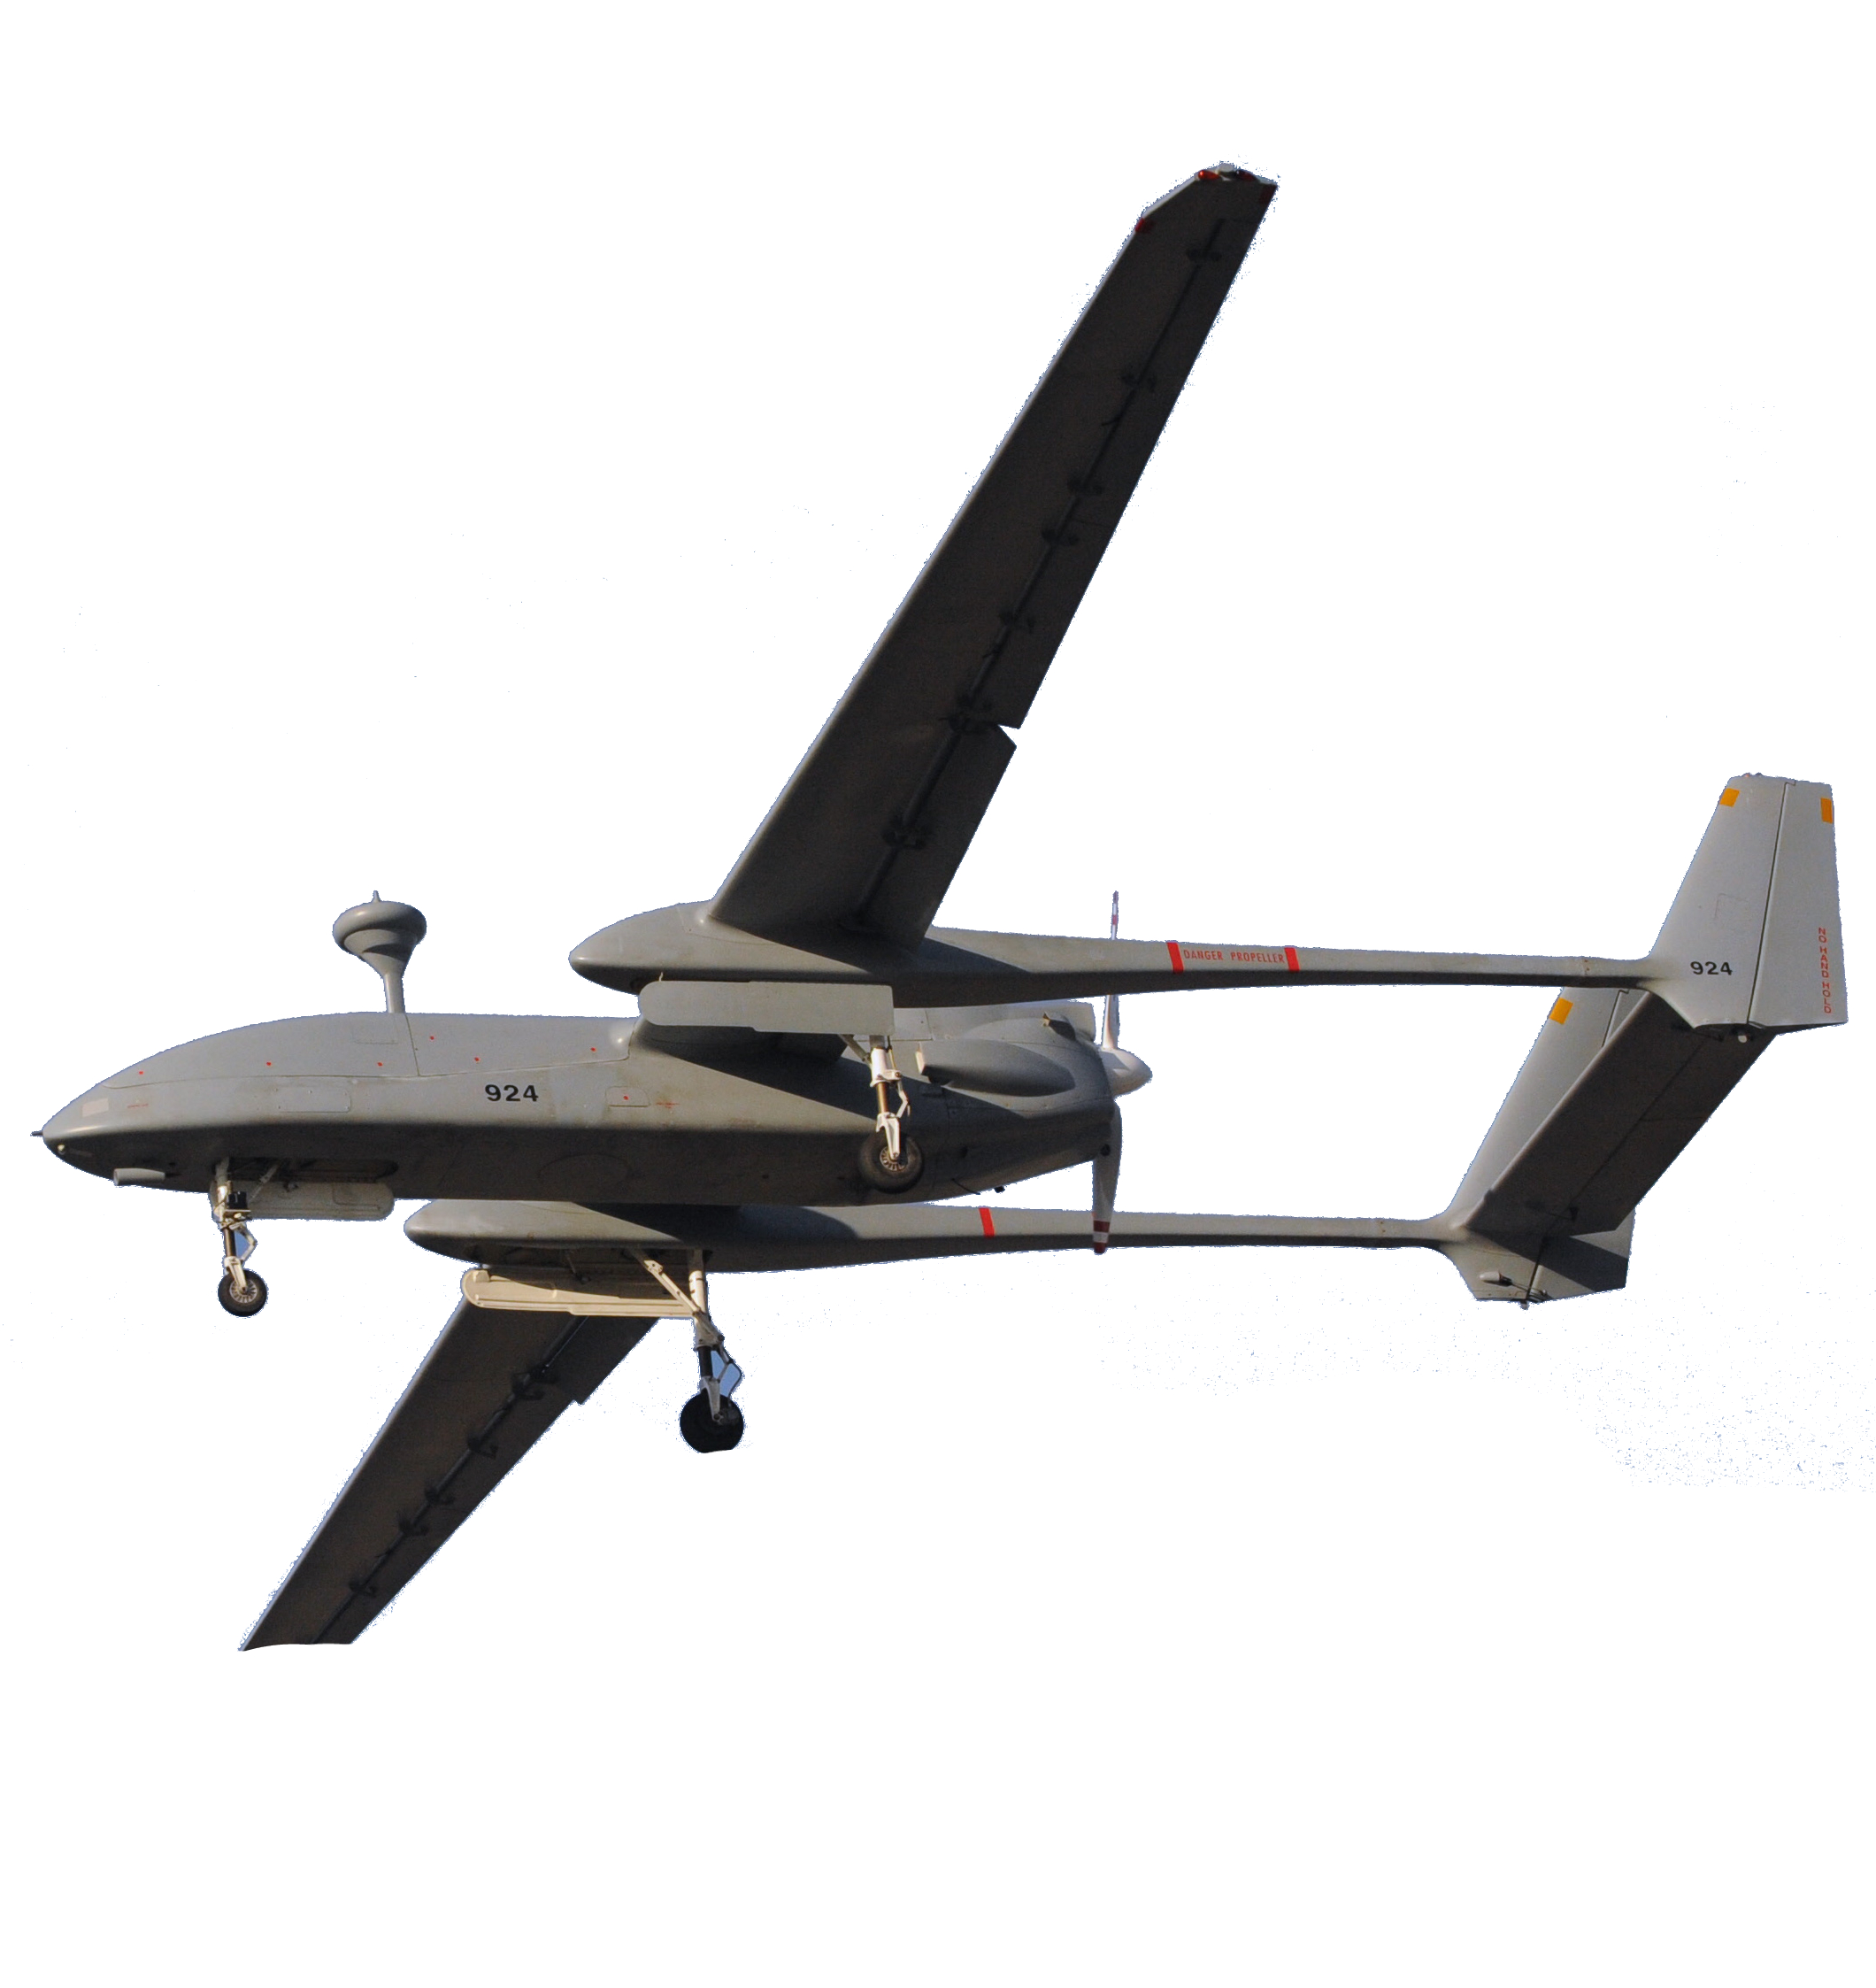
\includegraphics[height=4.1cm]{drone}}
\logodeux{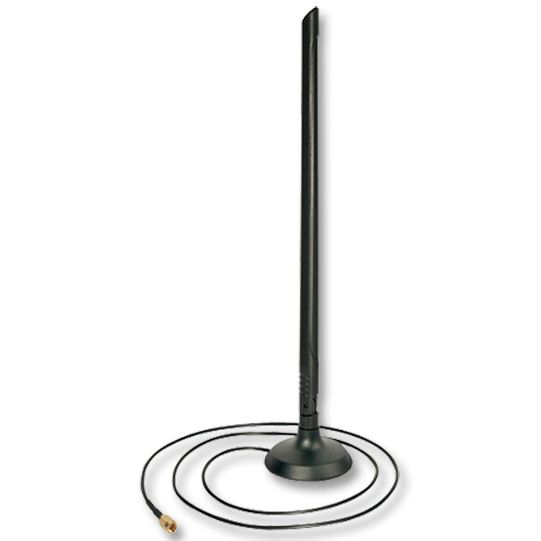
\includegraphics[height=4.2cm]{antenne}}



%%%%%%%%%%%%%%%%%% DEBUT DU DOCUMENT
\begin{document}

\maketitle
\thispagestyle{empty}
\newpage

\tableofcontents


%%%%%%%%%%%%%%%%% INTRODUCTION

\chapter*{Introduction}
\addcontentsline{toc}{chapter}{Introduction}


\newpage	  
%%%%%%%%%%%%%%%%%%%%%%%%


\chapter{Contexte}

\section{Nature du besoin}

Les drones sont de plus en plus présents dans le monde moderne est font maintenant partie intégrante du paysage urbains. Il est en effet possible d'acheter pour 50\euro~  un drone miniature dans n'importe quel rayon de jouet de grandes surfaces comme Leclerc, Carefour, Géant Casino, ... %Mais son usage ne s'arrête pas au loisir, de grandes firmes américaines comme Amazon souhaite utiliser ces drones pour livrer leur produit
Mais son usage ne s'arrête pas au loisir puisque l'actualité a montré que l'intrusion de drones dans des sites sécurisés représentaient un risque de sécurité majeur.

Notre projet au nom de SMART (System with Multi Antennas to Reorient a Target) doit répondre a ce problème en proposant une solution de détection de drone. Pour cela nous allons utiliser un système passif qui réceptionne les ondes émises par le drone puis utilise l'effet Doppler sur ces ondes pour obtenir la direction d'émission. Ainsi grâce a deux dispositif il sera possible d'obtenir la position du drone a détecter. 




%%% Local Variables: 
%%% mode: latex
%%% TeX-master: "../rapport"
%%% End: 

\chapter{Ingénierie Système}

\section{Analyse Fonctionelle}

\subsection{Diagramme Pieuvre}

Le diagramme pieuvre permet de mettre en évidence rapidement la fonction principale du système et les principales contraintes qui s'appliquent sur le système. Ce dernier est représenté par l'ovale central et l'ensemble des éléments extérieurs ayant une influence sont matérialisés tout autour. Les différentes relations sont appelées les fonctions de contraintes qui naissent d'une contrainte imposée par un élément extérieur « météo », de l'existence d'un produit déjà existant « un autre drone émettant des ondes » ou encore d'une exigence particulière de l'utilisateur voire de la présence de normes et de législations, de limitations lié au budget ou du type d'alimentation énergétique nécessaire.


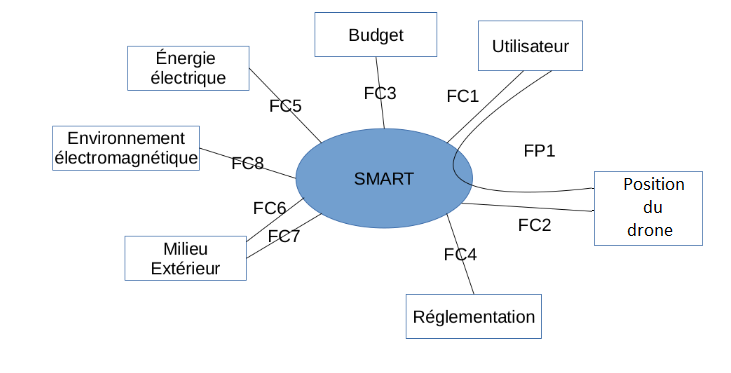
\includegraphics[width=0.90\textwidth]{Diagramme_pieuvre_corr.png}
\captionof{figure}{Diagramme pieuvre}


\subsection{Diagramme FAST}

Ce diagramme  présente la  manière de penser et d'agir. Le diagramme FAST se construit de gauche à droite, dans une logique du pourquoi au comment. On développe les fonctions de service du système en fonctions techniques. On choisit des solutions pour construire finalement notre système. On a mentionné les fonctions techniques chacune  à part pour trouver la solution convenable qui nous permet à la fin la réalisation finale du système. En utilisant des outils et méthodes déjà existant, on a trouvé des solutions qui satisfont les fonctions demandés.
L’antenne goniomètre était l’une des solutions les moins chères pour la détection du drone, à condition d’avoir au minimum deux antennes pour préciser la position et la vitesse du drone. Dès la détection du drone, il sera alors possible de déterminer sa position, d'enregistrer cette position via un logiciel dédié (MATLAB)

~\\

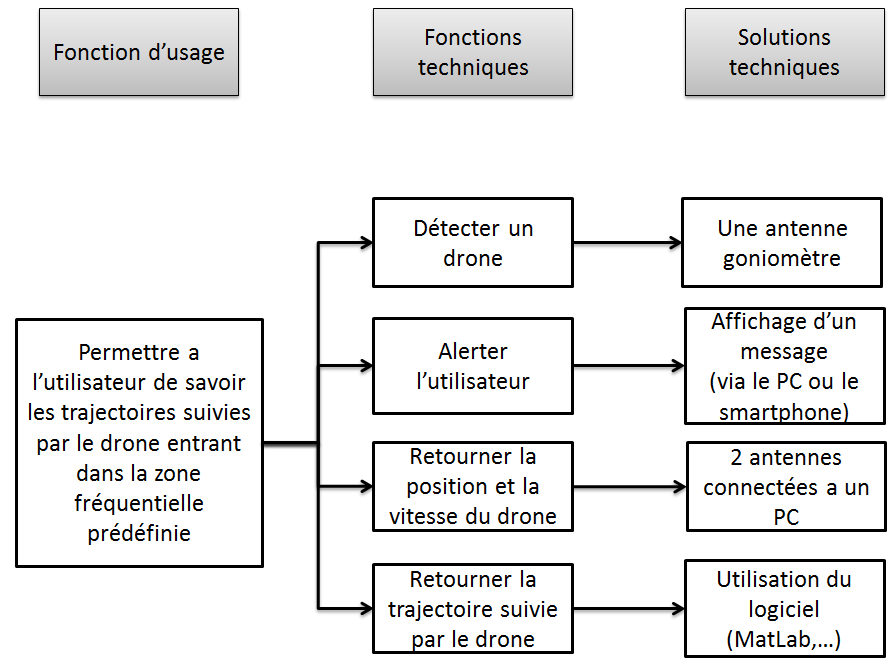
\includegraphics[width=1\textwidth]{FAST.png}
\captionof{figure}{Diagramme pieuvre}

%%% Local Variables: 
%%% mode: latex
%%% TeX-master: "../rapport"
%%% End: 
\chapter{Réalisation}

%%% Local Variables: 
%%% mode: latex
%%% TeX-master: "../rapport"
%%% End: 


%%%% CONCLUSION %%%%%%%%%

\chapter*{Conclusion}
\addcontentsline{toc}{chapter}{Conclusion}
\newpage

%%%% ANNEXE %%%%%%%%%%%%

\part*{Annexe}
\appendix
\nocite{*}
%\input{annexe_}
\newpage
 \listoffigures
 \printindex
 \bibliographystyle{frplain}
  \bibliography{biblio}

\end{document}
%%%%%%%%%%%%%%%%% FIN DU DOCUMENT
